\chapter{Architecture du projet}

\section{L'image du mode recovery}

\subsection{L'image de base}
le mode recovery se base sur le kernel linux 2.6.35.3 qui est contenu dans une ROM interne à la liseuse (il est donc inaccessible). Le sytème de fichier est compris dans un fichier image contenu lui sur la carte SD, ce fichier peut être modifié depuis l'extérieur.

L'image fournit par default pour le mode recovery, contient : 
\begin{itemize}
	\item un exécutable busybox \\
		qui permet l'accès aux commandes usuelles linux dans les systèmes embarqués
	\item un serveur dhcp
	\item un daemon telnet
	%peut etre a mettre dans la partie du rapport intermediaire
	\item un accès au port usb en mode série (via le module g_serial)
\end{itemize}

Busybox est un exécutable reprenant toutes les commandes usuelles linux pour les environnements
embarqués.

Le système de fichier du mode recovery est en lecture seule, seul les dossier suivant sont accessible en lecture écriture : 
\begin{itemize}
	\item /etc
	\item /initrd/mnt/sd
	\item /tmp
\end{itemize}

Pour modifier le système de fichier racine il faut passer par un pc hôte.

\subsection{L'image finale}

L'image finale ajoute les fonctionnalités suivante à l'image : 
	\begin{itemize}
		\item un accès au port usb par connexion Ethernet
		\item le support du protocole SSH
		\item la librairie DirectFB
	\end{itemize}

Plusieurs fonctionnalités devenues inutiles ont été désactivé :
\begin{itemize}
	\item Le serveur dhcp : \\
		il est peut utile d'avoir un support dhcp alors que le pc hôte et la liseuse 
		ont un réseau pour eux seuls.
		%peut etre rajouté le fait qu'il sont en plus défini statiquement ??
	\item Le daemon telnet : \\
		la gestion du protocole telnet est devenue inutile et peut pratique (la copie de fichier
		 n'étant pas gérer par exemple), depuis l'ajout du support du protocole SSH.
\end{itemize}

L'émulation d'un lien Ethernet sur le port usb de la liseuse se fait via le module g_ether.
%a verifier si c'est pas déjà dis avant
Ce module est située comme les autres modules dans :
	\begin{lstlisting}
	/lib/modules/2.6.35.3/kernel/drivers/usb/gadget
	\end{lstlisting}

Le support du protocole SSH se fait via la l'exécutable dropbear situé dans : 
	\begin{lstlisting}
	/bin
	\end{lstlisting}

Les fichiers concernant la librairies DirectFB se situe dans le dossier /usr/local/lib.
Pour pouvoir lancer une exècutable utilisant DirectFB il faut vérifier que ce dossier soit bien inclus dans la variable d'environnement LD_LIBRARY_PATH, cette variable est défini dans le scripte rc.local.
\section{La mise en place de l'affichage}
%architecture pour affichage via directfb

L'affichage de la liseuse se fait grâce aux modules suivant : 
\begin{itemize}
	\item le driver mxc_epdc
	\item DirectFB
\end{itemize}~\\

Le driver se charge de faire les optimisation pour pallier au problème de réactivité de l'écran (via les tables LuTs notamment), ainsi que l'application des waveforms pour l'affichage sur l'écran.\\
Le driver fournit des ioctl pour permettre l'exécution des fonctionnalités du driver depuis l'espace utilisateur.~\\~\\
%verifier si c'est pas deja dis plus tot dans le rapport
DirectFB implémente des primitives graphique, comme le traçage de ligne. Ces dernières permettent de faire une abstraction sur le format du framebuffer.

Voici un schéma modulaire de l'application utilisant DirectFB : 

\begin{figure}[h!]
	\begin{center}	
		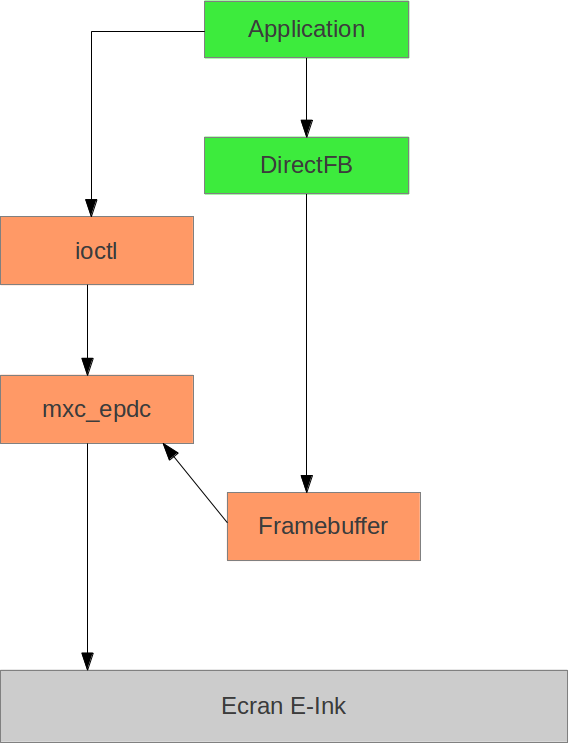
\includegraphics[scale=0.5]{schema_direct_fb.png}
		\caption{Architecture modulaire de l'application}
	\end{center}
\end{figure}

Dans l'état d'avancement actuel du projet, le programme met à jour le framebuffer via DirectFB et fait un appel ioctl au driver qui actualise l'écran en fonction du buffer. 
% application => directfb => framebuffer 				=> affichage
%						 => ioctl 	=> driver epdc   ||


%explication du fonctionnement 

% description de chaque module 
% directfb : abstraction du driver d'affichage
% ioctl : appel de la maj driver
%
%framebuffer